%&pdflatex
\documentclass[11pt]{article}
\usepackage{url,enumerate, amssymb, amsfonts}
\usepackage[colorlinks = true,
linkcolor = blue,
urlcolor  = blue,
citecolor = green,
anchorcolor = blue]{hyperref}
%\usepackage{setspace,listings}
\usepackage{graphicx}
\usepackage{amsmath}
\usepackage{psfrag}
\usepackage[font=small,labelfont=bf]{caption}
\usepackage{enumerate}
\usepackage{authblk}
\usepackage[sort&compress,comma,square,numbers]{natbib}
\usepackage{url} % not cruci
%\pdfminorversion=4
\usepackage{setspace}
\usepackage{lscape}
\usepackage{color,amssymb}
\usepackage{mathtools}
\usepackage{dcolumn}
\usepackage{indentfirst, verbatim, float}
\usepackage[margin=1.0in]{geometry}
%\newcounter{equationset, sectsty, breqn}
%\usepackage{setspace, amsmath,color}
%\usepackage{color,amssymb}
\usepackage{mathtools, amsthm, subcaption}
\theoremstyle{definition}
\newtheorem{definition}{Definition}[section]
\newtheorem{theorem}{Theorem}[section]
\newtheorem{corollary}{Corollary}[theorem]
\newtheorem{lemma}[theorem]{Lemma}
\newtheorem{remark}{Remark}
\bibliographystyle{unsrt}
\usepackage{sidecap}
\usepackage{titlesec}
\sidecaptionvpos{figure}{c}

% NOTE: To produce unblinded version, replace "0" with "1" below.
\newcommand{\blind}{0}
% DON'T change margins - should be 1 inch all around.
\newcommand{\cs}[1]{\textcolor{blue}{cs: #1}}

\begin{document}

\def\spacingset#1{\renewcommand{\baselinestretch}%
{#1}\small\normalsize} \spacingset{1}

%%%%%%%%%%%%%%%%%%%%%%%%%%%%%%%%%%%%%%%%%%%%%%%%%%%%%%%%%%%%%%%%%%%%%%%%%%%%%%
\title{\bf Nonparametric Network Dependence Testing by Diffusion Distance}
\if1\blind
{\author[1]{Youjin Lee (ylee160@jhu.edu)} %\thanks{cshen6@jhu.edu}}
	\author[2]{Cencheng Shen} %\thanks{cshen6@jhu.edu}}
	\author[2,3,4]{Joshua T. Vogelstein}
	\affil[1]{Department of Biostatistics, Johns Hopkins University}
  \affil[2]{Center for Imaging Science, Johns Hopkins University}
  \affil[3]{Department of Biomedical Engineering and Institute for Computational Medicine, Johns Hopkins University}
  \affil[4]{Institute for Data-Intensive Engineering \& Science, Johns Hopkins University}
	\maketitle
} \fi

	\if0\blind
	{
		\bigskip
		\bigskip
		\bigskip
		\begin{center}
			{\LARGE\bf Nonparametric Network Dependence Testing by Diffusion Maps}
		\end{center}
		\medskip
	} \fi

\begin{abstract}
%The text of your abstract. 200 or fewer words.
Investigating how network structures are associated with nodal attributes of interest is a core problem in network science. As the network topology is structured and often high-dimensional, many traditional nonparametric tests are no longer applicable and instead parametric approaches are dominant in network inferences. Here we propose a new procedure to testing dependence between network topology and nodal attributes. To deal with the structured data of network, we introduce a family of random vectors, called diffusion maps, which embed each node into the Euclidean space. The diffusion maps then provide network metrics which enable us to apply nonparametric distance-based correlation test. We demonstrate that our testing method, local optimal distance-based correlation test combined with proper network metrics, not only yields a consistent test statistic under common network models, but also significantly surpasses the testing power of existing benchmarks under various circumstances. 
\end{abstract}

\noindent%
{\it Keywords:} testing independence, exchangeable graph, diffusion distance, distance correlation, multiscale generalized correlation

\sloppy
\doublespacing

\section{Introduction}
\label{sec:intro}
	\vspace*{-0.2cm}
	% General Backgrounds
Propelled by increasing demand and supply of graph data from various disciplines, the ubiquitous influence of network inferences has motivated numerous recent advances and applications in statistics, physics, computer science, biology, social science, etc., which further poses many new challenges to data scientists. One of the most fundamental statistical questions is to determine and characterize the relationship among multiple modalities of a given data set, for which the first step is to test the existence of any dependency. However, the lack of a principal notion of correlation in the graph domain has not only hindered the progress of nonparametric dependency testing methods, but also deterred a rich literature of statistical techniques in other inferences (e.g., regression, feature screening, two-sample test) from being directly applied to graphs.
 
% Graph data general
Mathematically, a graph (or equivalently a network) $\mathbf{G}=(V,E)$ of sample size $n$ $(\in \mathbb{N})$ consists of a set $V$ of nodes (or vertices) together with a set $E$ of edges, which is often represented via an adjacency matrix $\mathbf{A} = \{A_{ij} : i,j= 1,..,n \}$, e.g.~for an unweighted and undirected network, $A_{ij} = 1$ if node $i$ and node $j$ are connected by an edge, and zero otherwise. Let $\mathbf{X} = \{  \mathbf{x}_{i} \in \mathbb{R}^{q_{x}} : i = 1, \ldots, n \}$ be nodal attributes, a random variable or random vector associated with each node. We assume that we are given an observed $n \times n$ adjacency matrix $\mathbf{A}$ and nodal attributes $\mathbf{X}$ for given $n$ nodes. Since $\mathbf{A}$ is a symmetric square matrix when $\mathbf{G}$ is undirected, it does not satisfy traditional data assumptions, e.g., each observation can be assumed independently and identically distributed, the sample size increases faster than the feature dimension, etc.. These are the notable obstacles for directly applying conventional statistical methods. Therefore, graph inferences have long relied on specifying a particular statistical model, such as the Erdos-Renyi model \cite{erdosrenyi1959,Gilbert1959}, stochastic block model~\cite{HollandEtAl1983, rohe2011spectral,SussmanEtAl2012,Lei2015} and its degree-corrected version \cite{karrer2011stochastic, ZhaoLevinaZhu2012}, the latent position model~\cite{TangSussmanPriebe2013,fosdick2015testing}, the random dot product model~\cite{YoungScheinerman2007, sussman2014consistent}, etc. 

However, model-based statistical methods often have limited applicability, e.g., connected-ness, unweighted-ness, and undirected-ness are the most common assumptions underlying statistical network models, which only represent a subset of real networks. Even under the model assumptions, how to select the model parameter can be expensive and unwarranted in practice, e.g., how to choose the dimension $q$ when assuming a latent position model. Moreover, model mis-specification can largely affect the inference performance on networks. It is thus desirable to develop robust graph analysis approaches that are less dependent on models and parameters \cite{ChenShenVogelsteinPriebe2016}.

% testing dependence on graphs
When it comes to investigating the relationships among network data, a core problem is to detect dependency between network topology and nodal attributes, i.e., certain properties defined on the nodes. For example, each person on Facebook not only has a number of distinct attributes (e.g., occupations, sex, personal behaviors), but also interacts with other persons via the social network; in neuro-science, each brain region has its own functionality, and is connected with other regions in the brain map. Identifying dependency between network and nodal attributes has also primarily focused on their relationship explained only by network model under the boundary of model assumption \cite{wasserman1996logit, fosdick2015testing, howard2016understanding}, thus suffers from the same problems all other model-based methods face. For example, the parametric network test proposed by Fosdick and Hoff \cite{fosdick2015testing} assumes a multivariate normal distribution of the latent factors as the generative model, estimates the latent factor of each node (which requires estimating $q$), then proceeds to test network dependence on the covariance by the likelihood ratio test. To our best knowledge so far, there is no principled method to compute a correlation measure on graphs, that is consistent and model-free and overcomes all existing restraints on network analysis. 

% Testing dependence
On the other hand, the general problem of dependence testing between two random vectors has seen notable progress in recent years. The Pearson's correlation~\cite{Pearson1895} is the most classical approach, which determines the existence of linear relationship via a correlation coefficient in the range of $[-1,1]$, with $0$ indicating no linear association while $\pm 1$ indicating perfect linear association. To capture all types of dependencies not limited to linear relationship, new correlation measures and nonparametric statistics have been suggested recently, such as the Mantel coefficient \cite{mantel1967}, RV coefficient \cite{RobertEscoufier1976}, distance correlation and energy statistic \cite{szekely2007measuring,szekelyRizzo2013a, RizzoSzekely2016}, kernel-based independence test \cite{GrettonGyorfi2010}, Heller-Heller-Gorfine (\texttt{HHG}) test \cite{HellerGorfine2013,heller2016consistent}, and multiscale generalized correlation (\texttt{MGC}) \cite{shen2016discovering}. In particular, the distance correlation by Szekely et al. \cite{szekely2007measuring} is the first correlation measure that is consistent against all possible dependencies (with finite moments), and the multiscale generalized correlation statistic by Shen et al. \cite{shen2016discovering} inherits the same consistency of distance correlation with remarkably better finite-sample testing powers under high-dimensional and nonlinear dependencies, via defining a family of distance-based local correlations and efficiently searching the optimal correlation in testing. Since all above methods are non-parametric, do not depend on particular models, and do not require explicit model parameter tuning, the network dependency testing may be significantly improved if some of them can be employed on graphs.

% proposed solution
To overcome the theoretical barricades by the distinct structure of network data, and to relax the limitations of model-based method for network testing, we come up with a solution that is theoretically sound and numerically superior: we first define a family of distance metrics on network data via the diffusion maps, then employ \texttt{MGC} to compute the optimal local correlation between the diffusion distance of the network topology and the Euclidean distance of the nodal attributes. Theoretical results show that the diffusion maps, acting as a node-wise representation, can allow distance-based correlation measures to be consistent in testing network dependencies under very mild condition, which includes almost all existing generative graph models, and regardless of the connected-ness, weighted-ness, and directed-ness of the graph. Moreover, the \texttt{MGC} statistic offers major power improvement under various scenarios in finite-sample testing. The combined advantages of diffusion maps and \texttt{MGC} over the existing benchmarks are illustrated via comprehensive simulations under popular network models.

	\vspace*{-0.2cm}
\section{Results}
\label{sec:method}
	\vspace*{-0.2cm}
\subsection{Diffusion Maps and Diffusion Distances}
\label{ssec:method2}

In this section, we introduce the diffusion maps as a family of network geometries for a graph \cite{coifman2006diffusion}, and show that they can yield node-wise conditional \textit{i.i.d.} samples for an exchangeable graph as sample size increases to infinity.

Coifman and Lafon~\cite{coifman2006diffusion,lafon2006diffusion} proposed multiscale geometries of data called diffusion maps, which are constructed by iterating the transition matrix that determines the probability of moving forward from one node to the others during the random walk.  We are going to define such transition matrix $\mathbf{P}$ as $P_{ij} = A_{ij} / \sum\limits_{j=1}^{n} A_{ij}, i,j=1,\ldots,n$, but that it can be based on any reasonable kernels that represent the similarity between the node while satisfying the assumptions mentioned in ~\cite{coifman2006diffusion}. The diffusion maps at time $t$ are computed as follows : 
	\begin{align*}
	\mathbf{U}_{t} &=[ \mathbf{u}_{t}(1) , \ldots, \mathbf{u}_{t}(n) ]\\
    &= \begin{pmatrix} \lambda^{t}_{1} \phi_{1}(i), \lambda^{t}_{2} \phi_{2} (i), \cdots, \lambda^{t}_{q} \phi_{q}(i) \end{pmatrix}^{T} \in \mathbb{R}^{n \times q}.
	\end{align*}
where $\{ \lambda_{j} \}$ and $\{ \phi_{j}  \}$ are the non-zero eigenvalues and corresponding eigenvectors of the transition matrix $\mathbf{P}$, $q$ is the number of non-zero eigenvalues, $\lambda^{t}_{j}$ is the $t^{\mbox{th}}$~power of the eigenvalue, and ${\cdot}^{T}$ is the matrix transpose. Then diffusion maps locate each node's position at every diffusion time and provide node-wise multivariate coordinates through $\{\mathbf{u}_{t}(i)\}$.   

A graph $\mathbf{G}$ is called exchangeable if and only if its adjacency matrix $\mathbf{A}$ is jointly exchangeable \cite{orbanz2015bayesian}, i.e.,~for every permutation $\sigma$ of $n$ elements, $(A_{ij}) \stackrel{d}{=} (A_{\sigma(i) \sigma(j)})$. Exchangeability is a mild condition that most generative statistical network models satisfy, including all aforementioned models such as the stochastic block model and latent position model \cite{rohe2011spectral, sussman2014consistent, todeschini2016exchangeable}. Lemma~\ref{main_lemma} proves that the node-wise multivariate coordinates $\{ \mathbf{U}_{t} \}_{t \in \mathbb{N}}$ can furnish conditional \textit{i.i.d.} samples for vertices by an exchangeable graph, with the proof supplied in the Appendix.
\begin{lemma}[Conditional \textit{i.i.d.} of diffusion maps $\{\mathbf{u}_{t}(i)\}$]
	\label{main_lemma}
	Assume that $\mathbf{G}$ is an exchangeable random graph. Then as $n \rightarrow \infty$, the diffusion maps $\{ \mathbf{u}_{t}(i) : i = 1, \ldots, n \}$ are conditionally \textit{i.i.d.} given its underlying distribution.  
\end{lemma}

The \textit{diffusion distance} between each pair of nodes is then computed as the Euclidean distance of the diffusion maps. 
\begin{equation}
\label{eq:diffusion}
C^2_{t}[i,j]  :=   \parallel \mathbf{u}_{t}(i) - \mathbf{u}_{t}(j) \parallel   \quad i,j = 1,2, \ldots , n.
\end{equation}
As the diffusion time $t$ increases, the corresponding diffusion distance $C_{t}$ reveals the geometric structure of the network topology in a larger and larger scale, and is thus more likely to take into account of two nodes which are relatively difficult to reach each other. Figure~\ref{fig:diffusions} shows how well diffusion distance can better reflects the connectivity and exhibits the community structure in a graph (generated by the stochastic block model by Equation~\ref{eq:Three}), when a reasonable $t$ is chosen in the family of diffusion distances $\{ C_{t} : t \in \mathbb{N} \}$. Compared to adjacent relation or geodesic distance, diffusion distance better reflects the connectivity since it takes into account every possible path between the two nodes. 

Note that the diffusion distance can always be defined regardless whether the graph is connected or not, weighted or not, and directed or not. Although the parameter $t$ may seem like another model parameter to tune, in practice $t \in [3,10]$ usually yields similar inference results. Moreover, when combined with the \texttt{MGC} statistic later, the selection of $t$ only has a very small inference effect in testing power (due to the capability of \texttt{MGC} to locate the optimal local correlation). Therefore, throughout the paper we always take $t=5$ in simulations, and drop the subscript $t$ in the diffusion maps $\mathbf{U}$ from now on. 

\begin{figure}[ht]
	\centering
	\begin{subfigure}[b]{0.23\textwidth}
		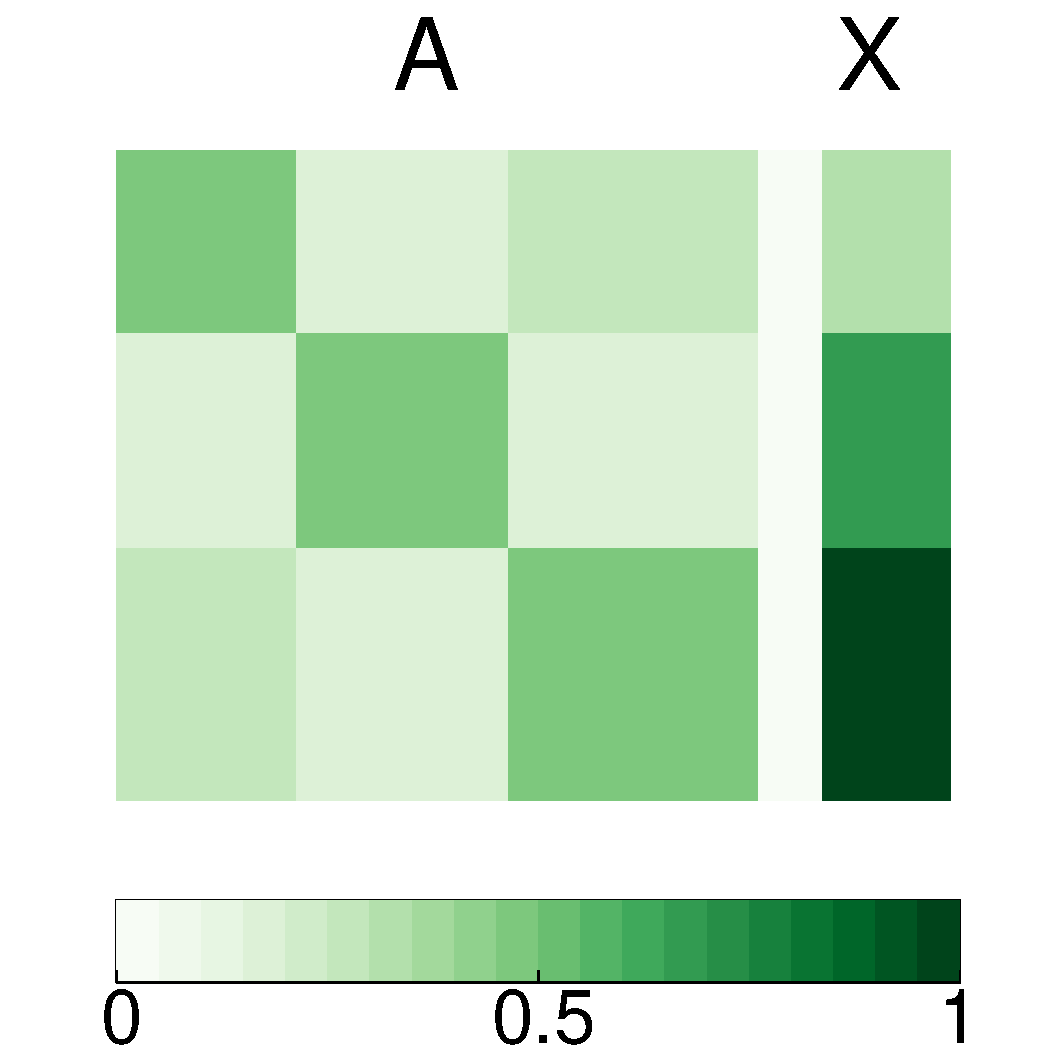
\includegraphics[width=\textwidth]{Pmat.pdf}
		\caption{}
		\label{fig:a}
	\end{subfigure}
	~ %add desired spacing between images, e. g. ~, \quad, \qquad, \hfill etc. 
	%(or a blank line to force the subfigure onto a new line)
	\begin{subfigure}[b]{0.23\textwidth}
		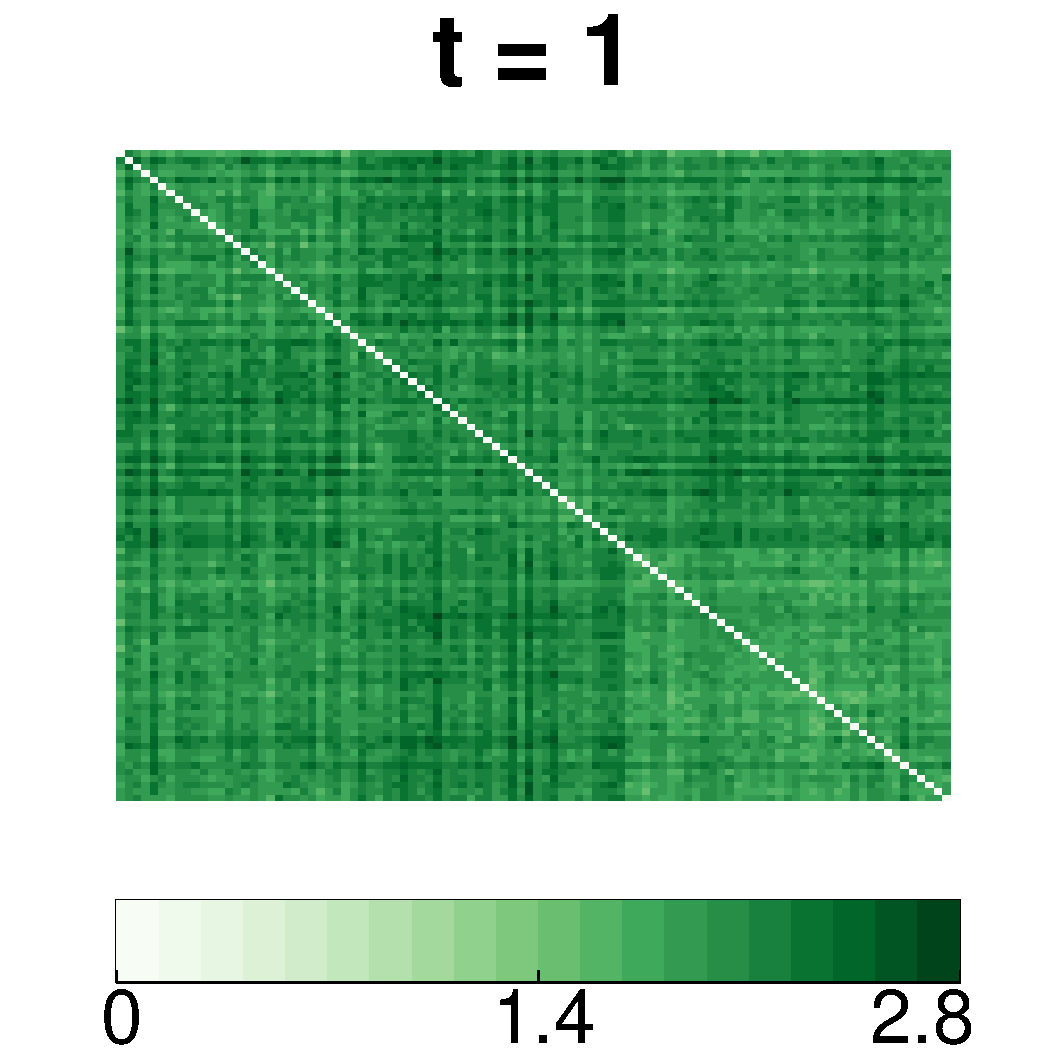
\includegraphics[width=\textwidth]{Dx1.pdf}
		\caption{}
		\label{fig:b}
	\end{subfigure}
	~ %add desired spacing between images, e. g. ~, \quad, \qquad, \hfill etc. 
	%(or a blank line to force the subfigure onto a new line)
	\begin{subfigure}[b]{0.23\textwidth}
		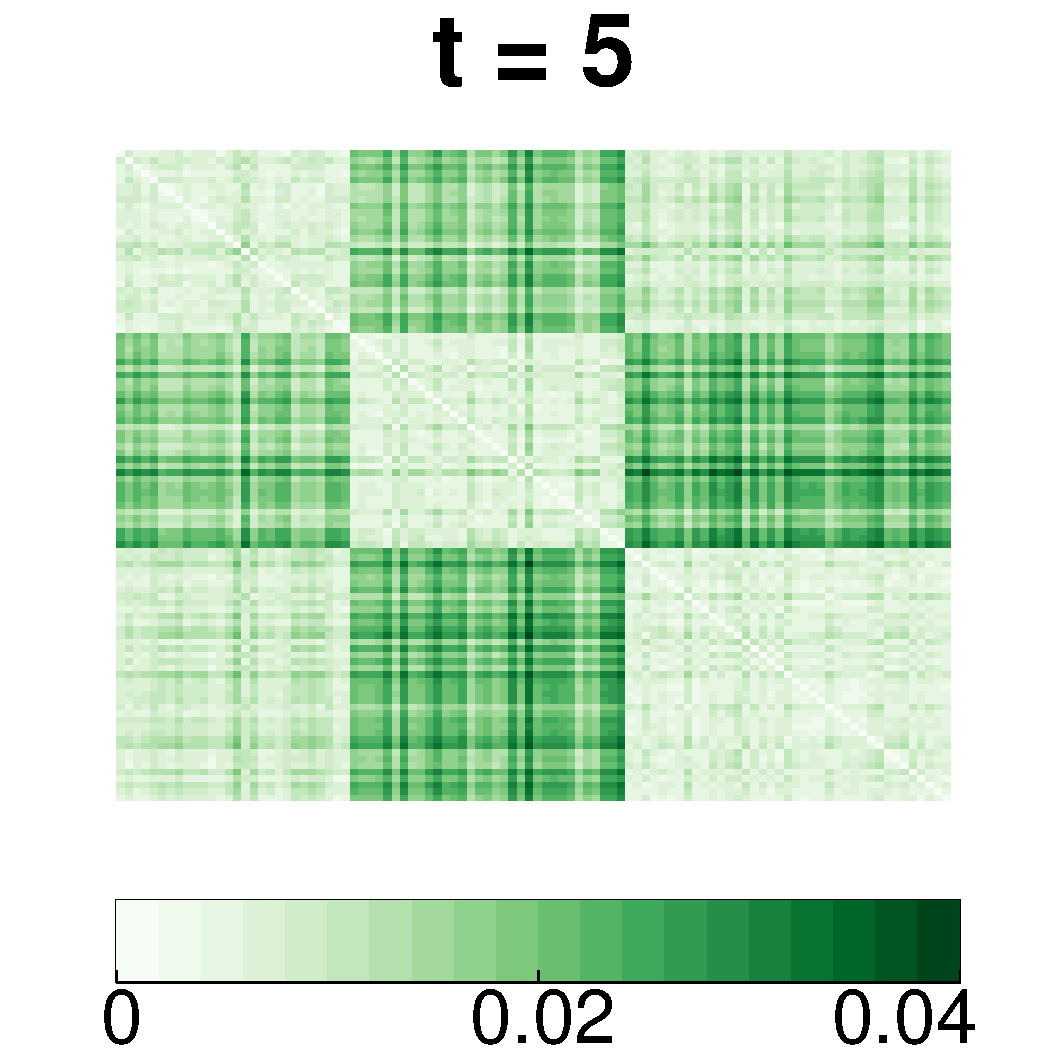
\includegraphics[width=\textwidth]{Dx5.pdf}
		\caption{}
		\label{fig:c}
	\end{subfigure}
	\begin{subfigure}[b]{0.23\textwidth}
		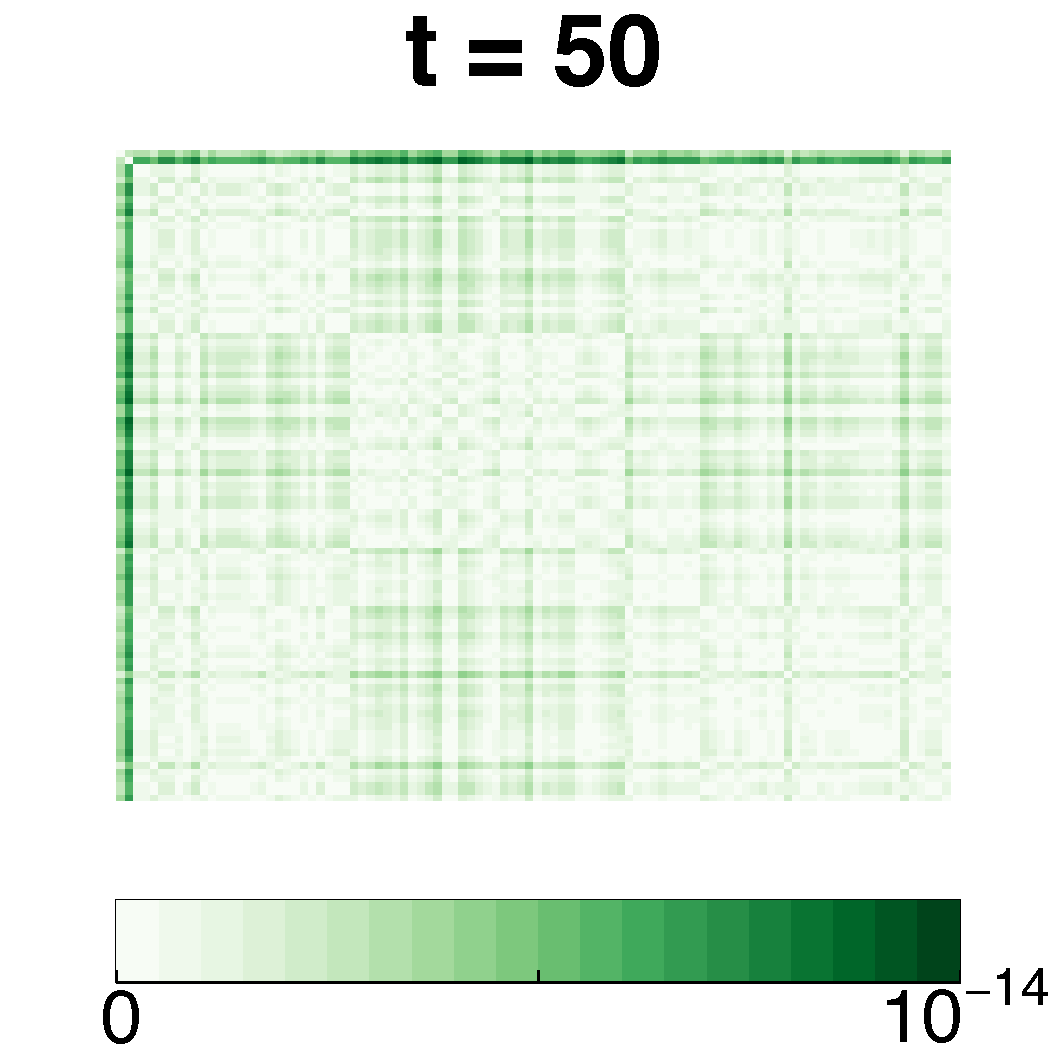
\includegraphics[width=\textwidth]{Dx50.pdf}
		\caption{}
		\label{fig:d}
	\end{subfigure}
	\caption{Panel (a) shows the adjacency matrix $\mathbf{A}$ and nodal attributes $\mathbf{X}$ Equation~\ref{eq:Three}. Panel (b), (c), (d) shows the diffusion distances of the graph, as a proposed network metric to provide a one-parameter family of network-based distances. As $t$ increases, there is a slight change in pattern, and the diffusion distance at $t = 5$ illustrates a very distinct block structures and thus a very clear dependency to the attributes $\mathbf{X}$.}
	\label{fig:diffusions}
\end{figure}

	\vspace*{-0.4cm}
\subsection{Dependence Testing via \texttt{MGC}}
\label{ssec:method1}
The results in Section~\ref{ssec:method2} allow us to cast the network dependency test into the following framework: given sample data $(\mathbf{U}, \mathbf{X}) = \{  (\mathbf{u}_{i}, \mathbf{x}_{i} ) ; i = 1,2, \ldots, n \}$ that are identically distributed as $(\mathbf{u},\mathbf{x}) \in \mathbb{R}^{q \times q_x}$ ($q$ and $q_x$ are the respective feature dimension), we are looking to test whether their joint distribution equals the product of the marginals, i.e.,
\begin{align*}
& H_{0}: f_{\mathbf{u}\mathbf{x}}=f_{\mathbf{u}}f_{\mathbf{x}},\\
& H_{A}: f_{\mathbf{u}\mathbf{x}}\neq f_{\mathbf{u}}f_{\mathbf{x}}.
\end{align*}

If $(\mathbf{u}_{i}, \mathbf{x}_{i} )$ can be further assumed independently distributed for each $i$, we can directly use a wide range of consistent test statistics, including the distance correlation, the \texttt{HHG} test, and \texttt{MGC}. Take the distance correlation for example: denote $C_{ij} = \parallel \mathbf{u}_{i} - \mathbf{u}_{j} \parallel$ and $D_{ij} = \parallel \mathbf{x}_{i} - \mathbf{x}_{j} \parallel$ for $i,j=1,2, \ldots ,n$, where $\parallel \cdot \parallel$ is the Euclidean distance. The sample distance covariance is defined as 
\begin{equation}	 
\label{eq:dCov}
\texttt{dCov}(\mathbf{U}, \mathbf{X}) = \frac{1}{n^2} \sum\limits_{i,j=1}^{n} \tilde{C}_{ij} \tilde{D}_{ij},
\end{equation}
where $\tilde{C}$ and $\tilde{D}$ is doubly-centered $C$ and $D$ by its column mean and row mean respectively, i.e., $\tilde{C}=HCH$, where $H=I_{n}-\frac{J_{n}}{n}$ (the double centering matrix), $I_n$ is the $n \times n$ identity matrix (ones on the diagonal, zeros elsewhere), and $J_n$ is the $n \times n$ matrix of all ones. The distance correlation \texttt{dCorr} follows by normalizing the distance covariance and is in the range of $[0,1]$. The best property of distance correlation is its consistency against almost all alternatives, i.e., $\texttt{dCorr}(\mathbf{U}, \mathbf{X})$ has testing power $1$ for $n$ large, for any joint distributions of finite moment. The \texttt{MGC} test inherits the consistency of distance correlation and significantly improves the finite-sample testing power via utilizing the correlation from a subset of data points. To be specific, we first compute all local correlations $c_{k,l}$ still based on the distance matrix of $\mathbf{U}$ and $\mathbf{X}$ but only including up to $k$-nearest points and up to $l$-nearest points for each data set. Then we locate the optimal local correlation, i.e., optimal choice of included neighborhood $(k^{*}, l^{*})$, which yields \texttt{MGC} statistic.

However, as the \textit{i.i.d.} assumption is not satisfied under network topology, the consistency of distance correlation is no longer guaranteed when applied to arbitrary distance metric of the graph. In particular, neither the Euclidean distance of the adjacency vector nor the shortest-path distance can work together with distance correlation without breaking its consistency proof. 

Using Lemma~\ref{main_lemma}, our next result shows that both the \texttt{dCorr} and \texttt{MGC} defined on the diffusion distance can have the same consistency when extended to network dependency test of exchangeable graphs.  

\begin{theorem}[\texttt{MGC} Consistency via Diffusion Distance]
Assume that $\mathbf{G}$ is an exchangeable random graph that is connected and unweighted, and its diffusion maps are $\mathbf{U}$ at certain $t \in \mathbf{N}$ with finite moment; and the nodal attributes $\mathbf{X}=\{ \mathbf{x}_{i}, i = 1,2, \ldots, n \}$ is \textit{i.i.d.} as a random vector $\mathbf{x}$ of finite moment. 

Then $\texttt{dCorr}(\mathbf{U}, \mathbf{X}) \longrightarrow 0 \mbox{ as } n \rightarrow \infty$ if and only if $\mathbf{U}$ is independent of $\mathbf{X}$. And both \texttt{MGC} and \texttt{dCorr} are consistent for testing dependence between any $\mathbf{U}$ and $\mathbf{X}$ satisfying the above condition.
	\label{theoremMain}
\end{theorem}

Therefore, our approach not only yields an easy-to-use methodology in network dependence testing, but also enjoys solid theoretical property and thus offers a principal approach to define correlation on network data. The proof of this theorem is postponed to the Appendix.

%Note that if $\{ \mathbf{w}_{i} : i = 1,2,\ldots, n \}$ are \textit{i.i.d}, they are also exchangeable. Thus estimated latent network factors, which are assumed \textit{i.i.d} by \cite{fosdick2015testing} can also be applied to Theorem~\ref{theoremMain}. We already have shown that even under undirected network, diffusion maps remain exchangeable at each diffusion time point $t$. 

%%%%%%%%%%%%%%%%%%%%%%%%%%%%%%%%%%%%%%%%%%%%%%%%%%
\section{Simulation Study}
\label{sec:simulation}
	\vspace*{-0.2cm}
Next we investigate our approach via simulated models and empirical performances. In the simulation studies, we compare the empirical testing powers of four test statistics: \texttt{MGC}, \texttt{dCorr}, \texttt{HHG}, and the likelihood ratio test by Fosdick and Hoff (\texttt{FH})~\cite{fosdick2015testing}. For the first three statistics, we further consider three different metrics of the network topology: the Euclidean distances of the diffusion maps (\texttt{DM}), of each column of adjacency matrix (\texttt{AM}), and of the latent factors (\texttt{LF}, which is based on singular value decomposition of the adjacency matrix). The \texttt{FH} likelihood ratio test must always be based on the latent factors.

Note that all latent factors based methods require a selection of a dimension parameter $q$, which we vary $q \in [1,10]$ and take the optimal power within the range (e.g., as a benchmark, the \texttt{FH} test actually has its power maximized over the parameter range). While for the diffusion maps, it suffices to fix $t=5$ as discussed in Section~\ref{ssec:method2}.

For each simulation model and each test, we repeatedly generate sample graph and attributes for $500$ times, carry out the permutation test, and reject the null if the resulting p-value is less than $0.05$. The testing power of each method equals the percentage of correct rejection. We will mainly consider the stochastic block model (SBM) and its degree-corrected version for the simulation models, which are two major models used in community detection. 

Let us first consider SBM with $3$ blocks, i.e., partition the nodes into $3$ communities, and generate the edges by a Bernoulli random variable whose probability that is determined by the communities of the connecting nodes. Assume $n=100$ nodes whose class label $\mathbf{x}_i$ takes values in $0,1,2$ equally likely. The edge probability is designed as
\begin{equation}
\label{eq:Three}
E(A_{ij} | X_{i}, X_{j}) = 0.5 I(|X_{i} - X_{j}| = 0) + 0.2 I(|X_{i} - X_{j}| = 1) + 0.3 I(|X_{i} - X_{j}| = 2), \quad i,j = 1, \ldots, n = 100.
\end{equation} 
Namely, within-block edge probability is $0.5$, between-block edge probability is $0.2$ or $0.3$ depending on the communities. This 3-block model describes a nonlinear dependency, where \texttt{MGC} has been shown to work better than the \texttt{dCorr} given a pair of random vectors~\cite{shen2016discovering}. We want to assure the performance of \texttt{MGC} given a graph object and a random vector of nodal attributes, coupled with a proper metric. A visualization of one sample graph is offered in Figure~\ref{fig:diffusions}. After repeatedly data generation and hypothesis testing by all methods, the powers are computed and shown in Figure~\ref{fig:threeSBM}, for which \texttt{MGC} combined with diffusion maps indeed yields the most superior power comparing to all other benchmarks.

\begin{SCfigure}[][ht]
	\centering
	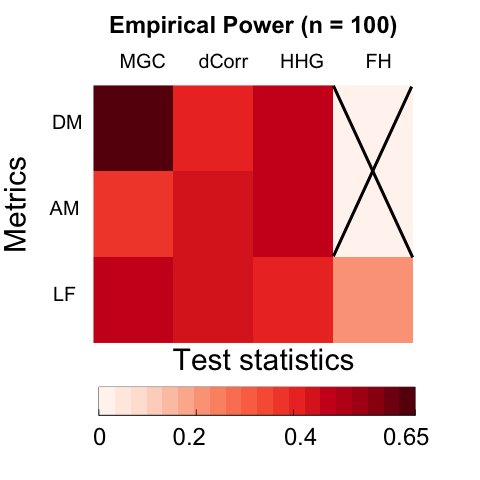
\includegraphics[width=0.4\paperwidth, height=0.4\paperwidth]{ThreeSBM_results_short.png}
	\caption{The power heatmap under SBM with three blocks, for all possible combinations of test statistics with distance metrics. \texttt{MGC} with the diffusion maps yields the best power comparing to all other methods. }
	\label{fig:threeSBM}
\end{SCfigure}

To further understand the advantage of \texttt{MGC}, next we fix the diffusion distance as the metric, and compare different test statistics. Based on the same three-block model, the edge probability is now generated as follows, by controlling the amount of \textit{nonlinear dependency} through $\theta \in (0, 1)$:
\begin{equation}
E(A_{ij} | X_{i}, X_{j}) = 0.5 I(|X_{i} - X_{j}| = 0) + 0.2 I(|X_{i} - X_{j}| = 1) + \theta I(|X_{i} - X_{j}| = 2), \quad i,j = 1, \ldots, n = 100.
\label{eq:mono}
\vspace*{-0.4cm}
\end{equation}
When $\theta > 0.2$, the network dependency changes from a close to linear relationship to strongly nonlinear. Figure~\ref{fig:powerplot} shows the testing power with respect to increasing $\theta$, and there is a clear trend that both the \texttt{dCorr} and \texttt{FH} tests have deteriorating power while \texttt{MGC} has a very stable performance against varying $\theta$. The same phenomenon holds by varying other edge probabilities. Therefore, \texttt{MGC} can better capture the nonlinear dependencies for network dependence testing, and is the best method to couple with the diffusion distance.
\begin{figure}[ht]
	\centering
	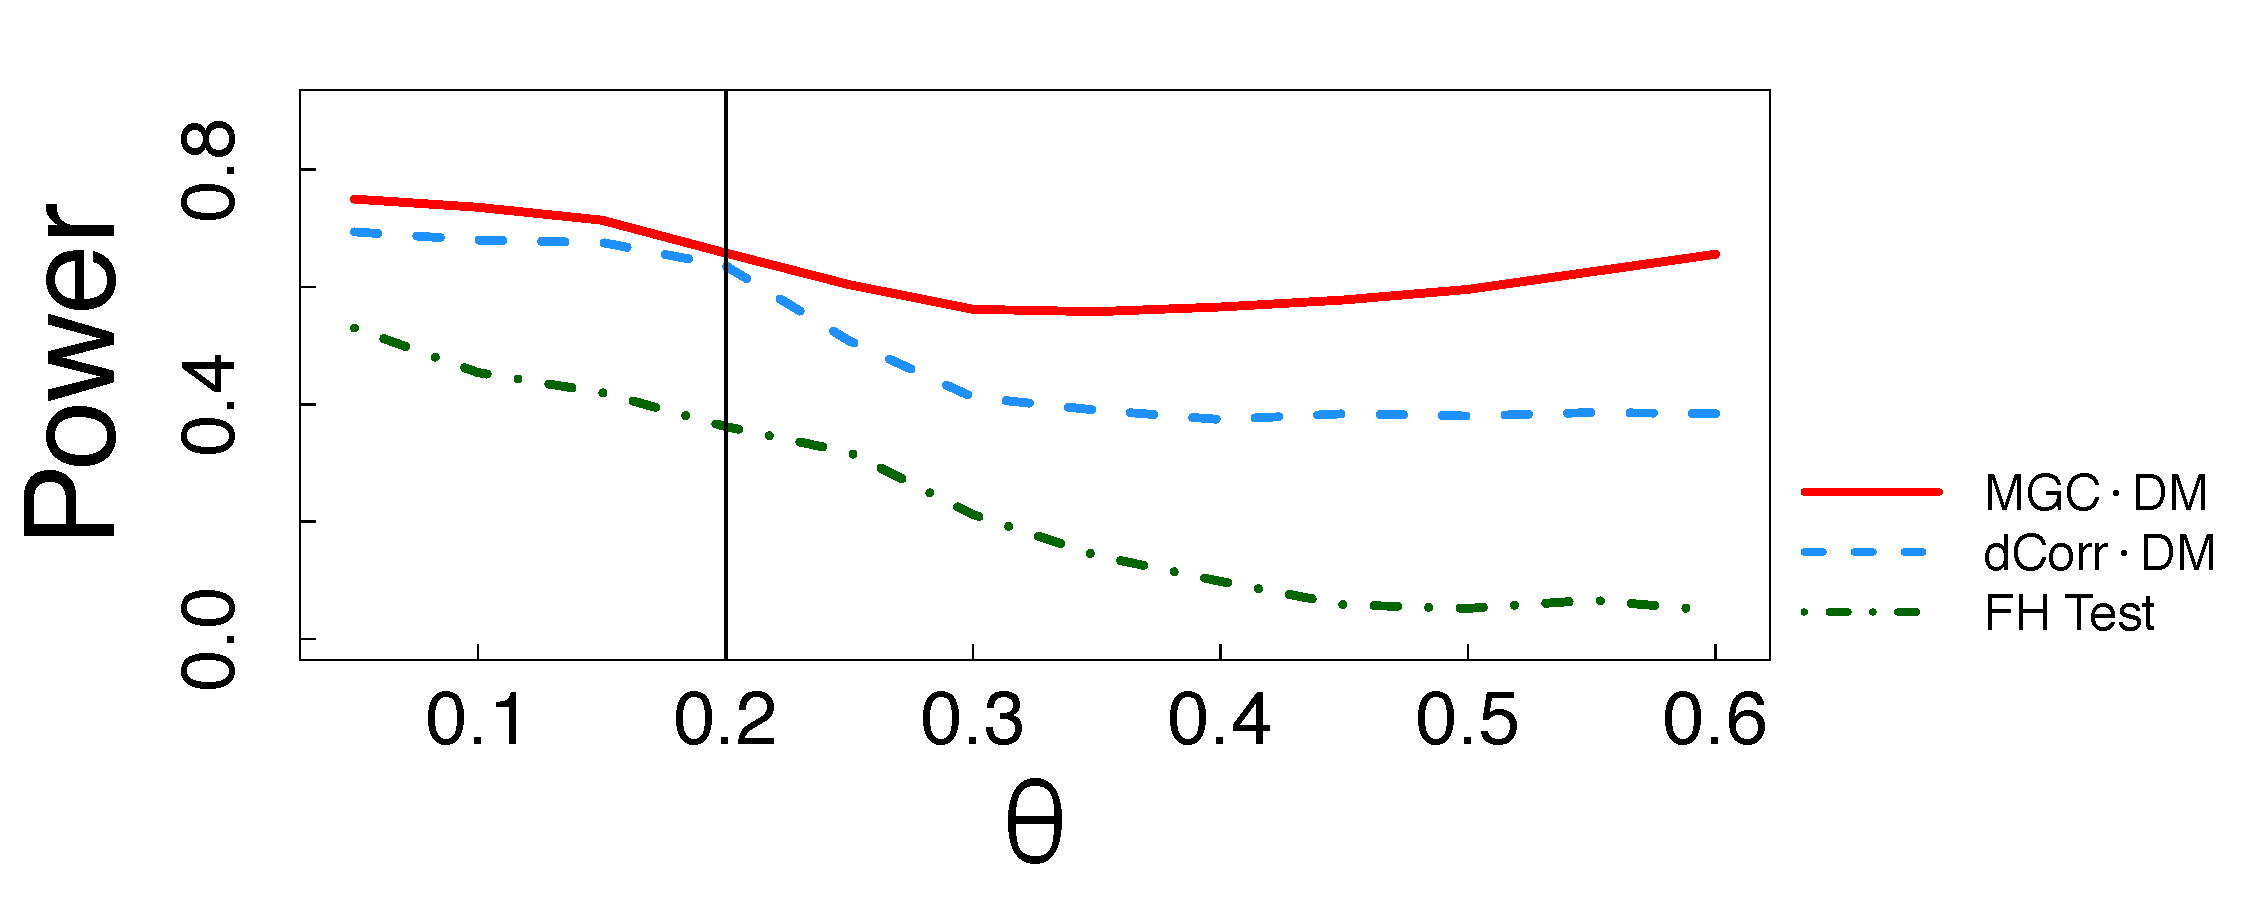
\includegraphics[width=0.7\linewidth]{mono_short.pdf}
	\caption{The power curve with respect to increasing $\theta$ in SBM with three blocks, for \texttt{MGC}, \texttt{dCorr}, and \texttt{FH}. Larger $\theta$ implies stronger nonlinear dependency, while $\theta<0.2$ has close-to-linear dependency. \texttt{MGC} is the best performing method throughout all possible $\theta$.} 
	\label{fig:powerplot}
\end{figure}

% degree-corrected two block model
Our next simulation shifts to the degree-corrected stochastic block model (DCSBM) with two blocks. DCSBM adds another random variable $V_{i}$ associated with each node to vary the node degrees, which is a generalization of the stochastic block model and provides a better fit to real networks. Suppose $n=250$, the nodal attributes / class label $X_i$ takes values in $0$ and $1$ equally likely, and the edge probabilities are specified by  
\vspace*{-0.4cm}
\begin{equation}
E( A_{ij} | \mathbf{X}, \mathbf{V} )  = 0.2 V_{i} V_{j} \cdot I ( |X_{i} - X_{j}| = 0 ) + 0.05 V_{i} V_{j} \cdot I(|X_{i} - X_{j}| = 1),
\label{eq:tau}
\vspace*{-0.4cm}
\end{equation} 
where $V_{i} \overset{i.i.d}{\sim} Uniform(1 - \tau, 1 + \tau)$ for $i = 1, \ldots, n$, and $\tau$ is a parameter to control the amount of variability of the edge distribution. Again, $\texttt{MGC} \circ \texttt{DM}$ is the best method in power throughout $\tau$ (not shown); and in Figure~\ref{fig:dcSBM} we show the testing power restricted to $\texttt{MGC}$ but varying the distance metrics, which shows the diffusion distance is indeed the best distance metric for network dependence testing.

\begin{figure}[ht]
	\centering
	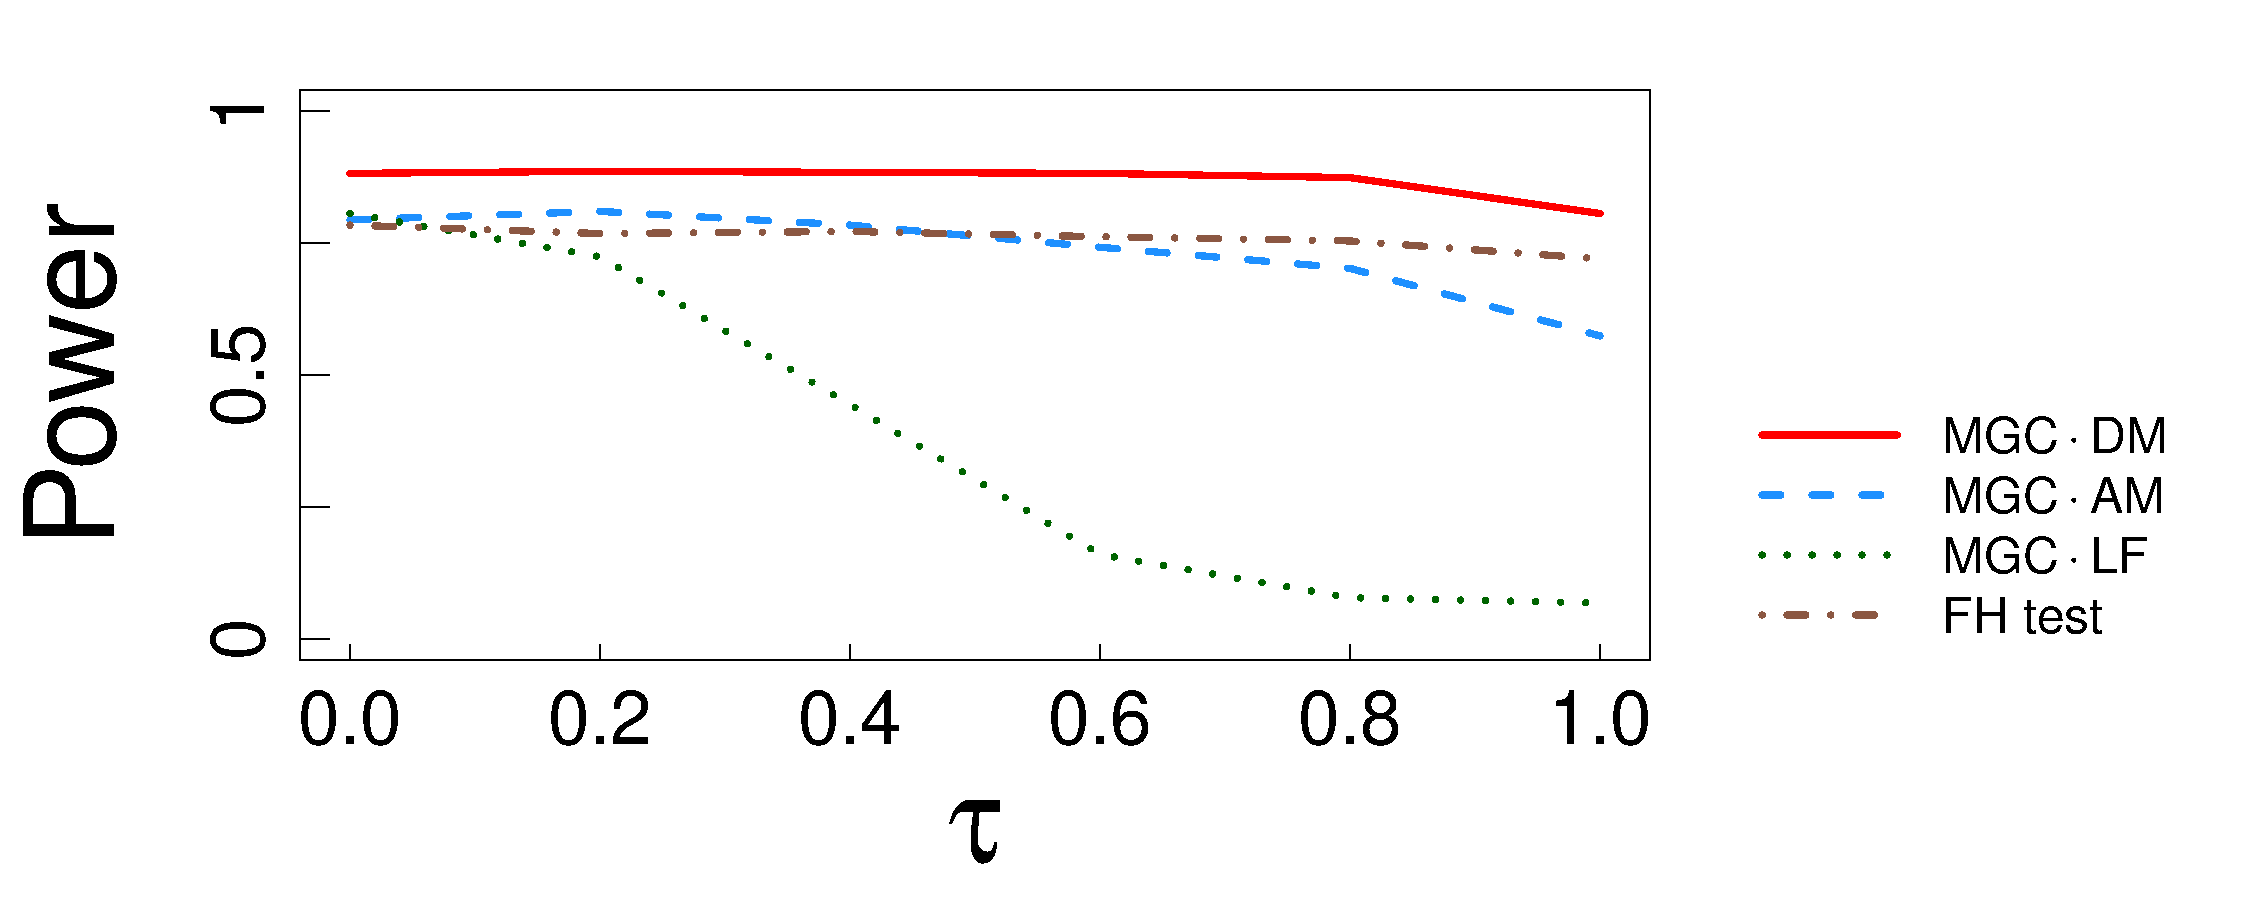
\includegraphics[width=0.7\linewidth]{tau_short.pdf}
	\caption{The power curve with respect to increasing $\tau$ in DCSBM with two blocks, for \texttt{MGC} with different distance metrics and \texttt{FH}. The diffusion distance exhibits the best testing power comparing to other metrics, and is better than the \texttt{FH} test.}
	\label{fig:dcSBM}
	\vspace*{-0.5cm}
\end{figure}

%%%%%%%%%%%%%%%%%%%%%%%%%%%%%%%%%%%%%%%%%
%\section{Real Data Examples}
%\label{sec:real}
%\begin{figure}[ht]
%	\centering
	%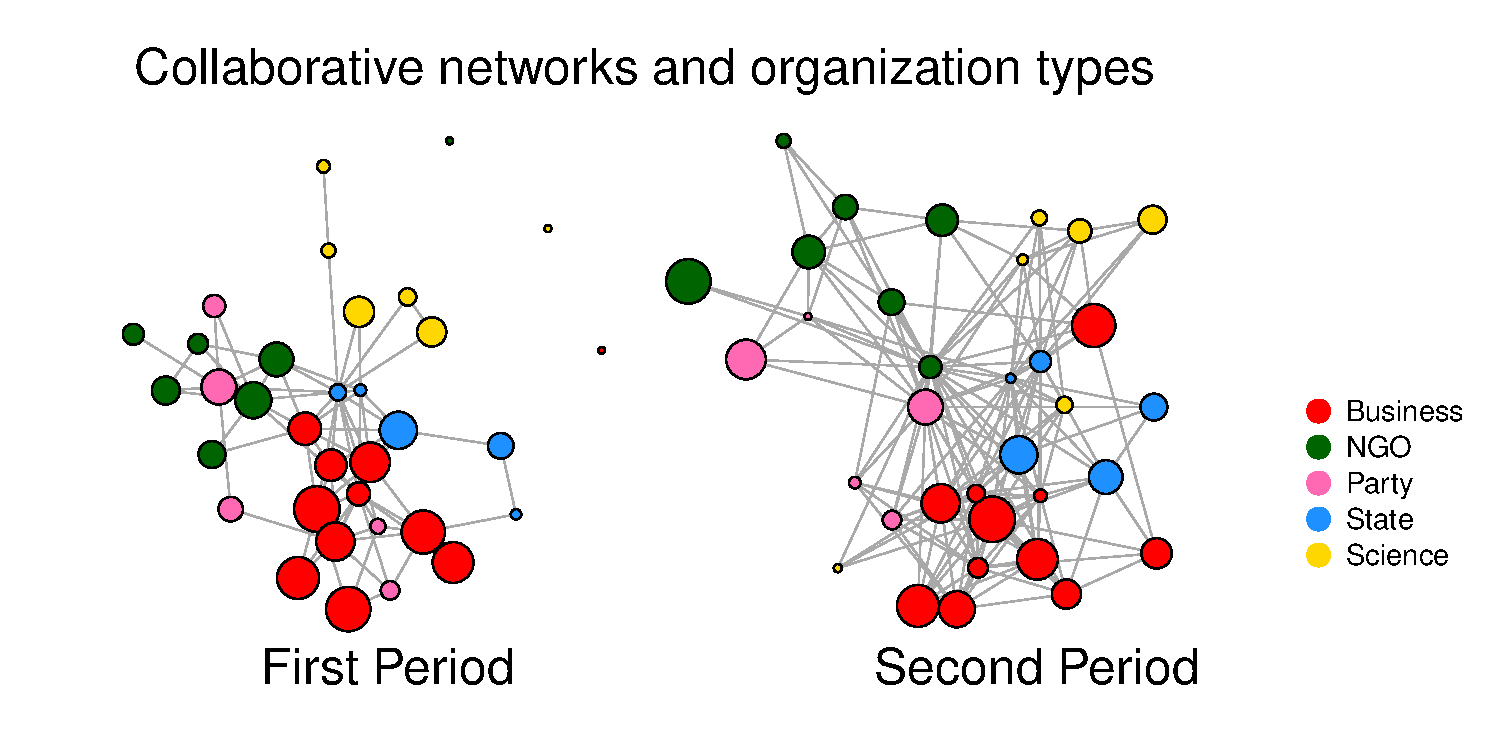
\includegraphics[width=\linewidth]{../Figure/two_politics.pdf}
	%\caption{Both panels depict the collaborative networks during the two time periods having significant network dependency in types of organizations. Using \texttt{MGC} statistics, we are not only able to test network independence but also calculate each node's amount of contribution to detecting dependence, which is proportional to node size here. You can tell that the tendency to collaborate within the same type is strongest among the business group while scientist relatively collaborates less with any others, especially in the first period.}
	%\label{fig:politics}
%\end{figure}
%In the field of political science, who exerts more powerful impacts than the others over political network and which factors impact on the power differentials are one of the interests~\cite{ingold2014structural}. \cite{minhas2016inferential} made an inference from political networks~\cite{cranmer2016navigating} via the additive and multiplicative effects (AME). The AME model estimates the latent factors and uses them to test independence with the nodal attributes. Among diverse attributes that \cite{cranmer2016navigating} provided, we focus on the types of organizations and how 34 political organizations having different types are participating policy network. We changed a given directed network into undirected network and use a dissimilarity matrix for distance matrix of the attributes, i.e., $\parallel \mathbf{X}_{i}  - \mathbf{X}_{j} \parallel = 0$ if and only if node $i$ and node $j$ are from the same type and one otherwise. Two collaboration networks comprised of the same set of nodes across two time periods are provided~\cite{ingold2014structural}. Figure~\ref{fig:politics} and Figure~\ref{fig:barplots} illustrates these two networks and shows each node's reliance on its organization type when collaborating. During the two periods, the network independence test statistics of \texttt{MGC} (p-value : (0.002 , 0.002)) and \texttt{dCorr} (p-value : ( 0.000, 0.000)) using diffusion distance matrices result in significant p-values across diffusion times from $t=1$ to $t=10$. The conclusion from the \texttt{FH} test (p-value : ( 0.000, 0.000)) is also the same.  
%\begin{figure}[ht]
	%\centering
	%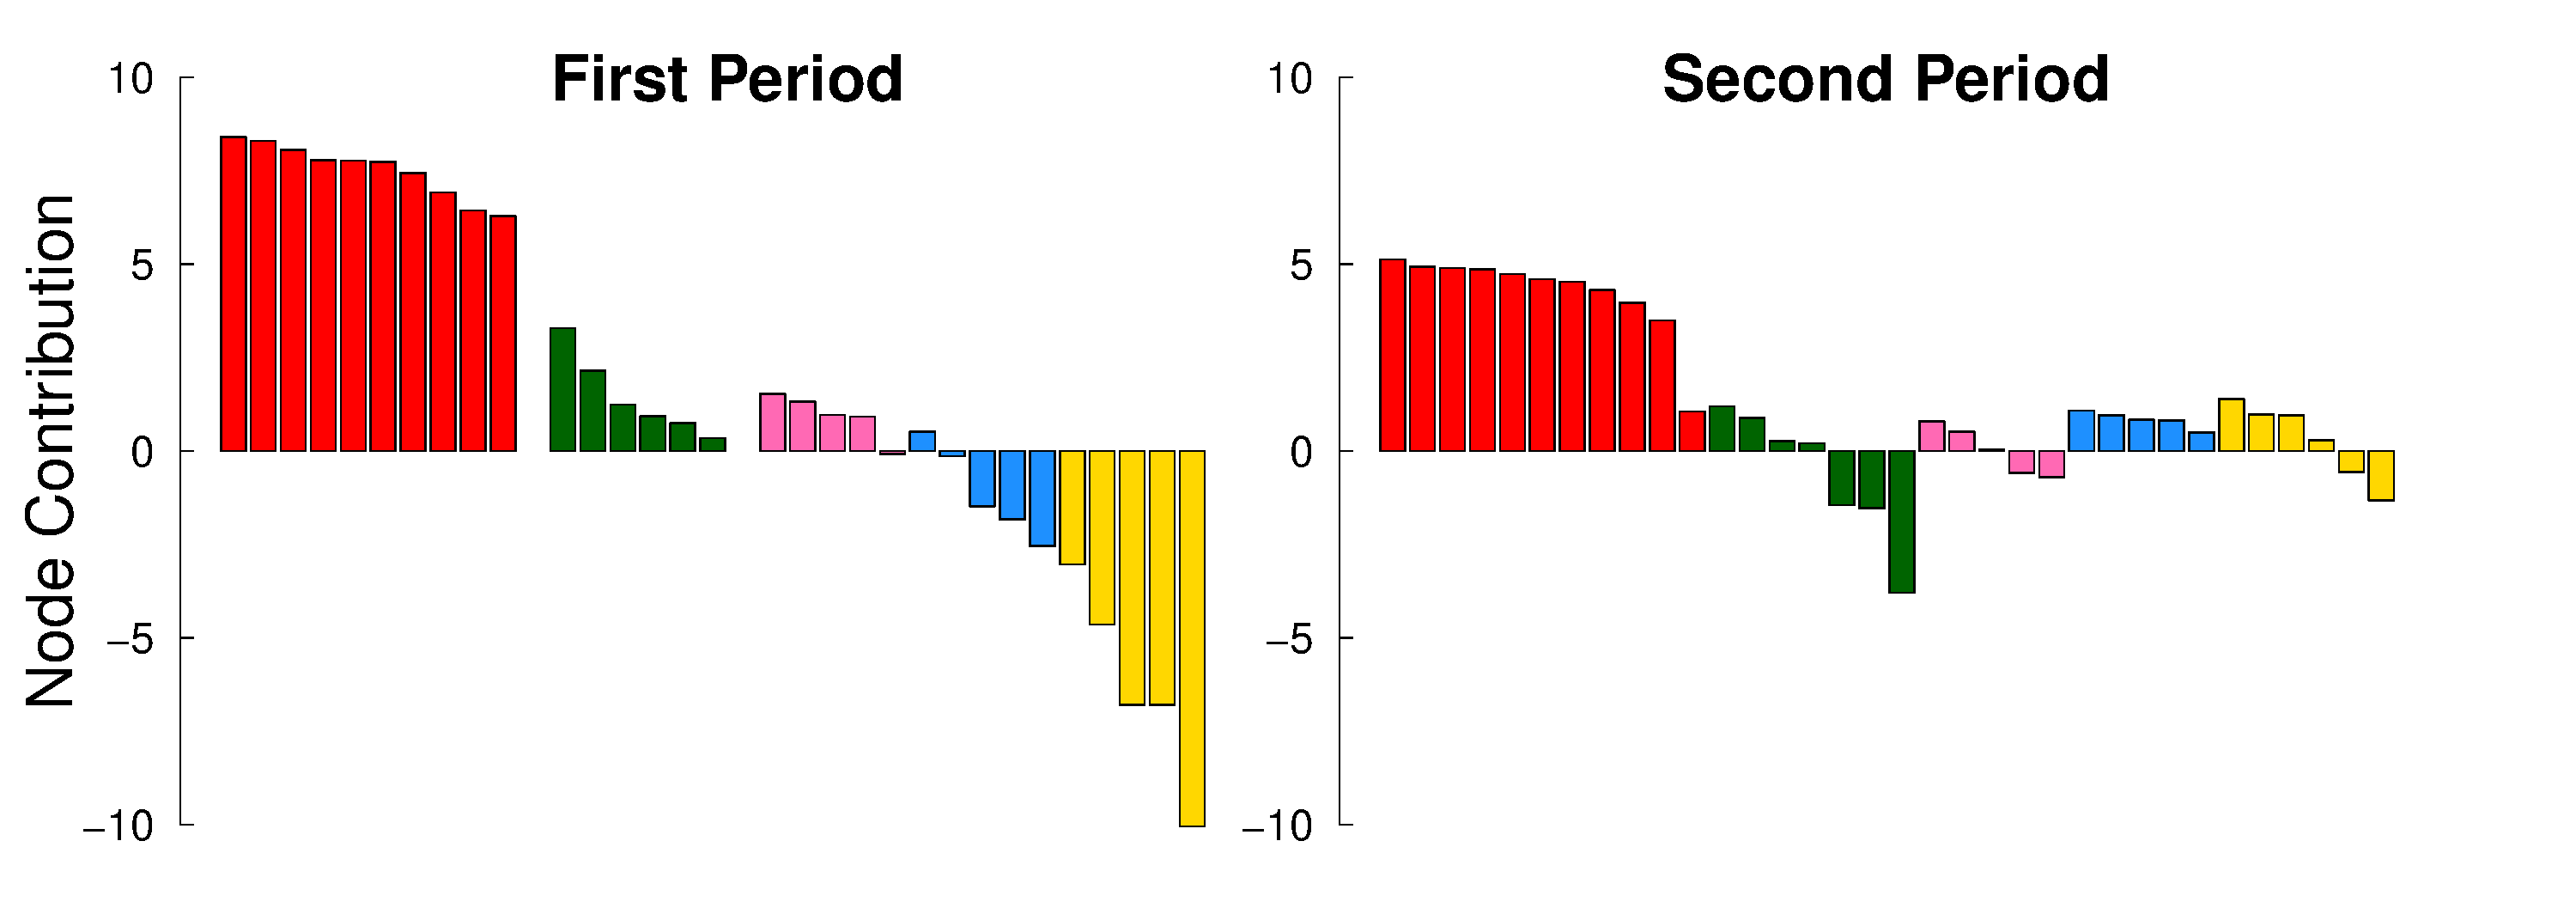
\includegraphics[width=\linewidth]{../Figure/barplots_nolegend.pdf}	
	%\caption{In the first period, we have two extreme cases among the business group and science group, which reflects our observations in Figure~\ref{fig:politics}. Generally organizations cooperate more actively between different types in the second period but still their collaboration network is highly dependent on their organization types especially for business group.}
	%\label{fig:barplots}
%\end{figure}


%%%%%%%%%%%%%%%%%%%%%%%%%%%%%%%%%%%%%%%%
\vspace*{-0.5cm}
\section{Conclusion And Future Work}
\label{sec:conc}
	\vspace*{-0.2cm}
In this paper, we combined recent progress in dependency testing and metric learning into the graph domain, and showed that \texttt{MGC} on the diffusion distance offers an elegant and powerful solution to the network dependency problem, which overcomes many challenges and restraints in the domain of network analysis. We proved that our method is consistent under a mild condition inclusive of almost all popular graph models; and empirically demonstrated it has superior power over all benchmarks, with \texttt{MGC} and the diffusion distance being the core elements behind the success.

There are a number of additional potential extensions of this work. First, how to choose a better diffusion time $t$, or find a $t$ with provable finite-sample performance, may provide further insight into and establish a more solid foundation of this approach. Second, the network dependence testing here is actually equivalent to the two-sample test, i.e., whether two graphs come from the same distribution; thus our approach readily offers a new nonparametric two-sample test on networks, for which more investigation will bring a valuable addition to the graph analysis. Third, with a few alterations, the new correlation measure on graph may be utilized for other tasks, such as feature screening, outlier detections, clustering, and classification, etc. Fourth, as a next step of this paper, we will utilize this method to a wide range of graphs available in social network and brain analysis, to answer domain specific practical questions.

%convince that \texttt{MGC}, merged with a family of diffusion distance, provides us powerful independence test statistics in network. Having multiscale statistics, i.e.~one parameter family of statistics, is not avoidable because we regard distance between the nodes over network as a dynamic process. Through simulation studies, we demonstrate that our methods perform better than the others especially under nonlinear dependency, and we are able to measure each node's contribution to detecting dependency. Deriving the contributions is particularly important when there have possibly different amounts of the dependencies among the nodes.  

%However obtaining a full family of statistics are computationally infeasible. Also we did not suggest any theoretically supported tools to select one metrics among them so thus we have one single statistic. As an ad hoc, we selected an \textit{optimal} diffusion time $t$ with highest power from $t=1$ to $t=10$ for our simulation since we could observe a stabilized empirical power within this period. Developing the adaptive method to find this optimal $t$ where dependence is maximized would be a natural next step. Despite these shortcomings, we expect that we could also enjoy the properties of \texttt{MGC} and a family of diffusion distances in solving diverse problems which require to utilize local relationship of the data sets. For instance, we might be able to implement independence testing between two networks of same size by using diffusion distance of each network to investigate whether a pair of networks are topologically or structurally independent. This kind of work would shed light on revealing any relationship between the data sets which are not necessarily a random vector.

%%%%%%%%%%%%%%%%%%%%%%%%%%%%%%%%%%%%%%%%%%%%
\bibliography{reference}
%%%%%%%%%%%%%%%%%%%%%%%%%%%%%%%%%%%%%%%%%%%%%%
\section{Appendix}
\subsection{Proofs}
\label{ssec:proof}

%%%%%%%%%%%%%%%%%%%%%%%%%%%%%%%%%%%%%%%%	
\begin{proof}[\textbf{Proof of Lemma~\ref{main_lemma}}]
	To prove conditional \textit{i.i.d.} of $\{\mathbf{u}(i)\}$ for $i=1,\ldots,n$ as $n \rightarrow \infty$, by the celebrated \textit{de Finetti's Theorem}~\cite{diaconis1980finite}, it suffices to prove that $\mathbf{u}(i)$ for $i=1,\ldots,n$ are exchangeable, i.e., for any permutation $\sigma$, the permuted sequence $\mathbf{u}(\sigma(1)), \mathbf{u}(\sigma(2)), \ldots,\mathbf{u}(\sigma(n))$ distributes the same as the original sequence $\mathbf{u}(1), \mathbf{u}(2), \ldots,\mathbf{u}(n)$. Denote the permutation matrix as $\pi$, it is to show $\mathbf{U}$ always distributes the same as $\mathbf{U}\pi^{T}$ in matrix notation. 
	
	Recall that the diffusion map at time $t$ is represented as follows :
	\begin{align*}
	\mathbf{U} &=[ \mathbf{u}(1) , \ldots, \mathbf{u}(n) ]\\
    &= \Lambda \Phi^{T} \\
    &= \begin{pmatrix} \lambda^{t}_{1} \phi_{1}(i) & \lambda^{t}_{2} \phi_{2} (i)  & \cdots & \lambda^{t}_{q} \phi_{q}(i) \end{pmatrix}^{T} \in \mathbb{R}^{n \times q},
	\end{align*}
	where $\Lambda=diag\{ \lambda_{1},\lambda_2,\ldots,\lambda_q \}$ and $\Phi =[ \phi_1, \phi_2,\cdots,\phi_q ]$ are the diagonal matrix of non-zero eigenvalues and the corresponding matrix of eigenvectors of the transition matrix $\mathbf{P}$, i.e, $\mathbf{P}=\Phi \Lambda \Phi^{T}$. 
    
Given the graph $G$ is exchangeable, i.e., $A_{\sigma(i)\sigma(j)} \stackrel{d}{=} A_{ij}$, we have
				\begin{align*}
	\mathbf{P}_{\sigma(i) \sigma(j)} &= A_{\sigma(i) \sigma(j)} / \sum\limits_{j} A_{\sigma(i)\sigma(j)} \\
	  &\stackrel{d}{=} A_{ij} /  \sum\limits_{j} A_{ij} \\
		&= \mathbf{P}_{ij},
	\end{align*}
    from which it follows that
    \begin{align*}
	 \pi\mathbf{P} \pi^{T} &\stackrel{d}{=} \mathbf{P} \\
	  \Rightarrow (\pi \Phi) \Lambda (\pi\Phi)^{T} &\stackrel{d}{=} \Phi \Lambda \Phi^{T} \\
		\Rightarrow \mathbf{U}\pi^{T}= \Lambda (\pi\Phi)^{T} &\stackrel{d}{=} \Lambda \Phi^{T} = \mathbf{U}
	\end{align*}	
	Therefore, the diffusion maps are exchangeable, and also conditional \textit{i.i.d.} asymptotically.
\end{proof}

%%%%%%%%%%%%%%%%%%%%%%%%
\begin{proof}[\textbf{Proof of Theorem~\ref{theoremMain}} \texttt{MGC} Consistency via Diffusion Distance]

Assume that $(\mathbf{U}, \mathbf{X}) = \{ (\mathbf{u}_{i}, \mathbf{x}_{i}) ; i = 1,2, \ldots, n \}$ is identically distributed as $(\mathbf{u}, \mathbf{x})$. By \textit{Theorem 1} in \cite{szekely2007measuring}, we immediately have
\begin{eqnarray}
dCov(\mathbf{U},\mathbf{X}) &\longrightarrow \int_{D(\delta)}{\|g_{\mathbf{u},\mathbf{x}}^{n}(t,s)-g_{\mathbf{u}}^{n}(t)g_{\mathbf{x}}^{n}(s)\|^{2}}dw \quad \quad \mbox{ as } n \rightarrow \infty
\label{eq:conv1}
\end{eqnarray}
where $g_{\mathbf{u},\mathbf{x}}^{n}(t,s), g_{\mathbf{u}}^{n}(t), g_{\mathbf{x}}^{n}(s)$ are the sample characteristic functions, e.g., $g_{\mathbf{u},\mathbf{x}}^{n}(t,s)=\frac{1}{n}\sum_{j=1}^{n}\exp\{i \left\langle t,\mathbf{u}_{j} \right\rangle  +i \left\langle  s,\mathbf{x}_{j}\right\rangle \}$, and $w(t,s)$ is the weight function chosen in \cite{szekely2007measuring}. %This part holds without indepednent or finite moment assumption.

Lemma~\ref{main_lemma} shows that $\{ \mathbf{u}_{i} \}$ are conditional \textit{i.i.d.} for an exchangeable graph, i.e., there exists an underlying distribution random variable $\mathbf{u}$ such that $\mathbf{u}_{i}|\mathbf{u}$ are \textit{i.i.d.} as $n \rightarrow \infty$. By the strong law of large number for V-statistics \cite{KoroljukBook}, under finite moment assumption of $\mathbf{u}$ and $\mathbf{x}$, we have 
\begin{eqnarray}
\displaystyle\int_{D(\delta)}{\|g_{\mathbf{u},\mathbf{x}}^{n}(t,s)-g_{\mathbf{u}}^{n}(t)g_{\mathbf{x}}^{n}(s)\|^{2}}dw &\stackrel{n \rightarrow \infty}{\longrightarrow} 
\displaystyle\int_{D(\delta)}{\|g_{\mathbf{u},\mathbf{x}}(t,s)-g_{\mathbf{u}}(t)g_{\mathbf{x}}(s)\|^{2}}dw,
\label{eq:SLLN}
\end{eqnarray}
within a bounded circle $D(\delta)=\{(t,s):\delta \leq |t|_{p} \leq 1/\delta,\delta \leq |s|_{q} \leq 1/\delta\}$ for any $\delta>0$, where $g_{\cdot}(\cdot)$ is the population characteristic function, i.e., $g_{\mathbf{u},\mathbf{x}}(t,s) = E\{\exp\{i \left\langle t,\mathbf{u} \right\rangle  +i \left\langle  s,\mathbf{x}\right\rangle \}\}$. The same convergence still holds out of the circle $D(\delta)$, and a technical proof is in \textit{Theorem 2} of \cite{szekely2007measuring}.

Combining equation~\ref{eq:conv1} and equation~\ref{eq:SLLN} yields
\begin{eqnarray}
dCov(\mathbf{U},\mathbf{X}) &\longrightarrow \displaystyle\int{\|g_{\mathbf{u},\mathbf{x}}(t,s)-g_{\mathbf{u}}(t)g_{\mathbf{x}}(s)\|^{2}}dw,
\label{eq:main2}
\end{eqnarray}
which clearly equals $0$ if and only if independence holds. As distance correlation is just a normalized version of distance covariance, we also have 
\begin{eqnarray}
dCorr(\mathbf{U},\mathbf{X}) &\longrightarrow 0,
\label{eq:main1}
\end{eqnarray}
if and only if the diffusion maps $\mathbf{U}$ is independent of the nodal attributes $\mathbf{X}$.

By \cite{shen2016discovering}, Equation~\ref{eq:main1} holds under the same condition, when \texttt{dCorr} is replaced by \texttt{MGC}. Therefore, both \texttt{MGC} and \texttt{dCorr} are consistent in network dependence testing between the diffusion maps $\mathbf{U}$ and the nodal attributes $\mathbf{X}$.
\end{proof}
%%%%%%%%%%%%%%%%%%%%%%%%%%5
%\begin{proof}[\textbf{Proof of Theorem~\ref{theorem2}} Consistency of \texttt{MGC} applied to exchangeable variables]
	
%Under the exchangeability and finite second moment assumptions of underlying distribution, $\mathcal{V}^{2}_{n}(\mathbf{W},\mathbf{Y}) \xrightarrow{n \rightarrow \infty}  0$ if and only if underlying distribution of $\{\mathbf{w}_{i} \}$, $f_{\mathbf{w}}$ is independent from underlying distribution of $\{ \mathbf{y}_{i}  \}$, $f_{\mathbf{y}}$. Now suppose that we have undirected, connected network $\mathbf{G}$ with a family of diffusion maps $\{ \mathbf{u}_{t}  \}$ and with nodal attributes $\{ \mathbf{x}  \}$. We have shown in the Lemma~\ref{main_lemma} that $\{ \mathbf{u}_{t}  \}$ are exchangeable for each $t \in \mathbb{N}$. Thus there exists an underlying distribution of $\mathbf{u}_{t}$ such that $\mathbf{u}_{t}(i) \overset{i.i.d}{\sim} f_{\mathbf{u}^{(t)}}$ for each of $t= 1,2,\ldots $; and we have $\mathbf{x}_{i} \overset{i.i.d}{\sim} f_{\mathbf{X}}$. Under the assumption of finite second moment of $\mathbf{u}^{(t)}$ and $\mathbf{x}$, \texttt{MGC} statistics constructed by $\{  (  \mathbf{u}_{t}(i), \mathbf{x}_{i} ) : i = 1,2,\ldots, n  \}$ yield a consistent testing which determines the independence between underlying distributions of $\mathbf{u}^{(t)}$ and $\mathbf{x}$. From the same setting of network $\mathbf{G}$, we have estimated \textit{i.i.d} node-specific network factors $\{ \mathbf{F}_{i} \}$ so that $n$-pair of \textit{i.i.d} $\{ ( \mathbf{F}_{i}, \mathbf{x}_{i} )  \}$ can be applied to \texttt{MGC} or other distance-based tests without assuming conditioning underlying distribution. In case of using adjacency matrix directly into test, we must assume that the adjacency matrix comes from connected directed network, i.e. $A_{ij} \overset{i.i.d}{\sim} f_{A}$ for all $i,j=1,2,\ldots, n$; otherwise, each column is dependent on one another.  
%\end{proof}

\end{document}